\chapter{Workbook Assignment 1: Basic Probabilities and Visualisations}

\section{Bernoulli Distribution}
For each of the distributions below, please provide the requested graphics as well as the numeric results. In both cases, please provide how you realized these (calculations, code, steps…) and why it is the appropriate tools. Do not forget to include the scale of each graphics so a reader can read the numbers represented.

\section{Bernoulli Distribution}

Assumed a binary vote with outcome for or against is described by a Bernoulli distribution, with $P(vote = "for") = 0.69$. 
Interpreting this as a one-trial Bernoulli experiment with the two outcomes for and against - represented by success and no success respectively - we can visualize it as displayed in figure~\ref{fig:1a}.


\begin{figure}[h]
\centering
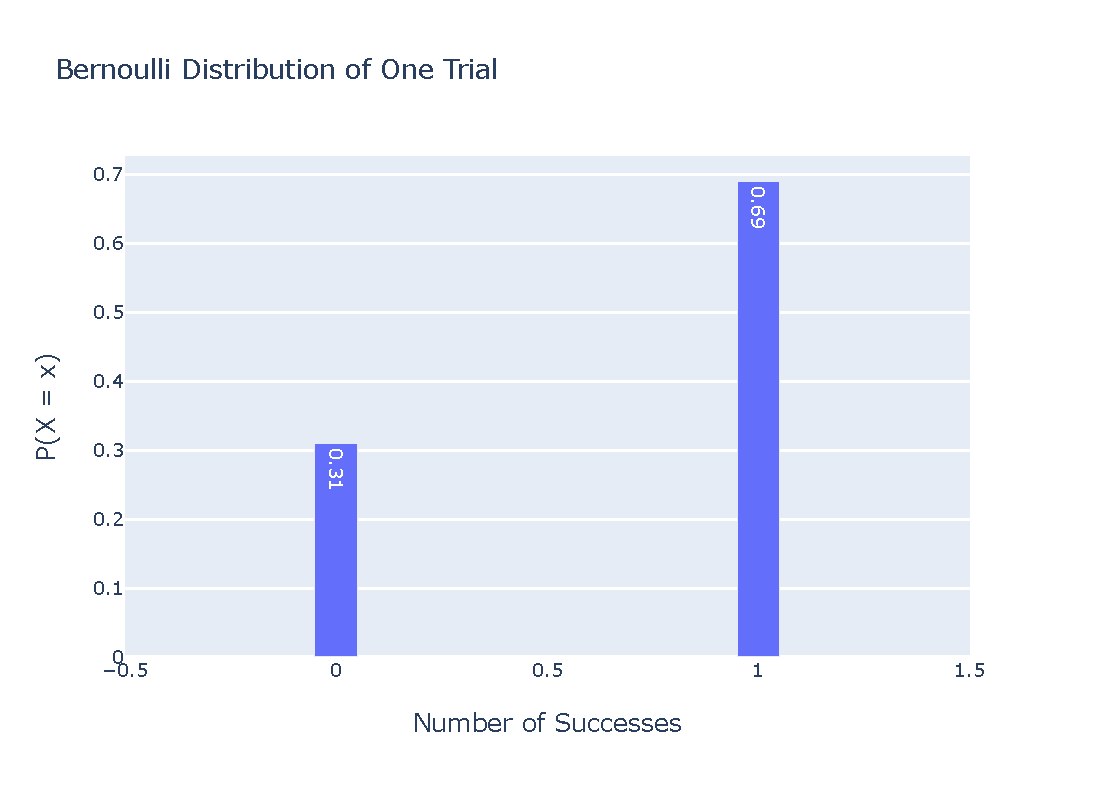
\includegraphics[width=16cm]{pics/1a.pdf}
\caption{Bernoulli Distribution of One Trial}
\label{fig:1a}
\end{figure}
\FloatBarrier


As this is a one-trial Bernoulli experiment, we can only observe the two outcomes $success = for$ and $no success = against$. With provided information that $P(vote = "for") = 0.69$, we can calculate that $P(vote=”against”) = 1 - P(vote = "for") = 0.31$. This is visualized by the two bars in figure~\ref{fig:1a}. 
For a Bernoulli experiment, the expected value is defined as p where p is defined as the probability of success on the trial CITATION HOGG. The probability of success in our case is p = 0.69 which is therefore our expected value. This means if we would repeat the experiment one hundred times, we expect to observe 69 successes. 



b) The number of meteorites falling on an ocean in a given year can be modelled by a Poisson distribution with an expectation or $\lambda$=37. Explain why a Poisson distribution is a natural candidate for this phenomenon. Give a graphic showing the probability of one, two, three… meteorites falling (until the probability is less than 0.5\%). Calculate the median and variance and show them graphically on this graphic.


c) Let $\Upsilon$ Y be the random variable with the time to hear an owl from your room’s open window (in hours). Assume that the probability that you still need to wait to hear the owl after �� hours is:
0.3e−0.5 ��+0.6e−0.25 ��
Find the probability that you need to wait between 2 and 4 hours to hear the owl, compute and display the probability density function graph as well as a histogram by the minute. Compute and display in the graphics the mean, variance, and quartiles of the waiting times.

\chapter{Workbook Assignment 2: Basic Probabilities and Visualizations }	

\section{Visualisation, Expectations and (Co)Variances}
Assumed you have recorded mappings of X and Y values, what is an appropriate way of visualisation and how do you find the sample covariance as well as the expectation values and variances per variable; assuming the data comes in the following format?\\
\\
(1.754, 720.15), (-7.385, -260.86), (1.396, -340.56), (-3.304, 954.75), 
(-12.159, -370.12),\\ (-6.767, -259.89), (1.233, 261.89), (-7.056, 400.72), 
(-1.222, -94.33), (-0.722, -492.02),\\ (-5.065, -789.42), (-9.333, 301.86), 
(7.27, -17.04), (-1.989, 257.91), (3.582, -229.89), \\(-1.2, -349.18), 
(4.118, 226.05), (-1.834, -534.54), (-1.882, 610.91), (8.677, 70.11) \\

As the variables in the data are both continuous and the question addresses the calculation of correlation, the optimal visualisation is a scatter diagram as for example figure~\ref{fig:WorkbookAssignment2a}.

\begin{figure}[h]
\centering
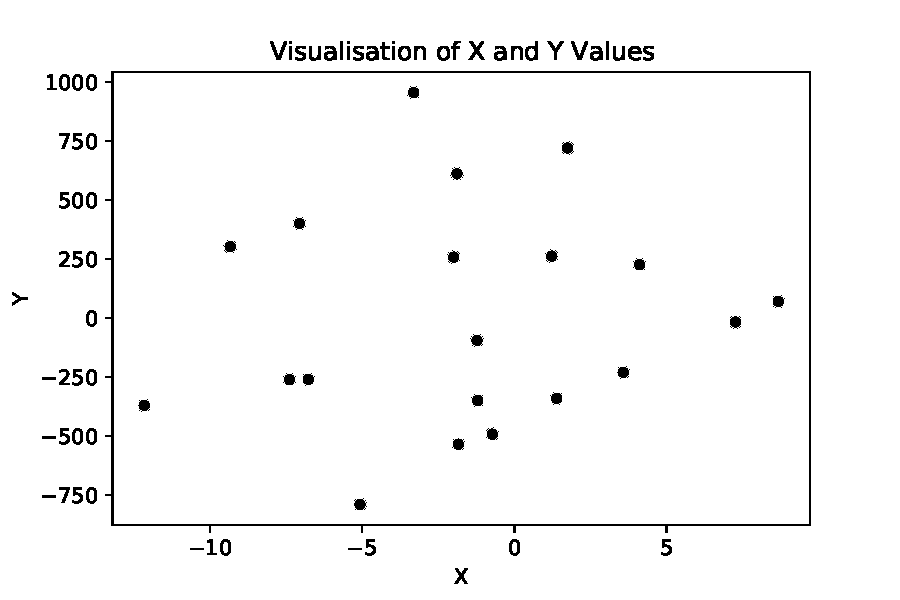
\includegraphics[width=16cm]{pics/WorkbookAssignment2a.pdf}
\caption{Visualisation of provided X and Y values as scatter plot}
\label{fig:WorkbookAssignment2a}
\end{figure}
\FloatBarrier

Looking at the scatter plot, one can observe that the data is quite evenly dispersed; No pattern can be determined at first glance. This rather evenly distributed data also suggests that the expected value for X and Y is rather close to 0. Calculating the expected value for each variable can be understood at the calculation of the expected value of a discrete random variable as the number of observations is discrete. Equation~\ref{eq:ExpValDiscrete} is therefore the formula to calculate the expected value. 


\begin{equation}  E(X) = \sum [x * P(x)]
\label{eq:ExpValDiscrete}
\end{equation}

http://mathcenter.oxford.emory.edu/site/math117/expectedValueOfADiscreteRandomVariable/
\\

The results are consequently $E(X) = -1.5944$ and $E(Y) = 3.3250$.

The sample covariance is defined in Equation~\ref{eq:COV}, where $\bar{x} = E(X)$ and $\bar{y} = E(Y)$ (adapted from~\cite{bruce2017practical}).

\begin{equation}  s_{xy} = \frac{\sum(x_{i}-\bar{x})(y_{i}-\bar{y})}{n-1}
\label{eq:COV}
\end{equation}

Applying the formula to the provided data, $s_{xy} = 284.23$ can be observed. This indicates a positive relationship, but does not provide any information on its quality. 

The calculations were done in Python, using NumPy, Pandas and Seaborn. The code for all calculations can be found in the appendices. 

\section{Ball throw}
b) Consider that a ball is thrown with a random angle $THETA$[0,360) (in degrees) and a random radius $r$ element of [0,1] (in meters) both independent and uniform. Calculate the density of the variable $X$ and $Y$ (the cartesian coordinates of the point at angle $THETA$ and radius $r$) as well as their expectation and variance.

Notes:
Only possible by transformation. if you know x yy dirstribution 
Monte carlo approach can solve this. (complicated)
Transformation theorem thingy 3.last chapter
For density, check Page 19 in skript. basically the pdf of a distribution






\chapter{Workbook Assignment 6: Bayesian Estimates}	

(following Hogg, McKean and Craig, exercise 11.2.2)
Let $X1, X2, ... , X10$ be a random sample from a gamma distribution with $\alpha =3$ and $\beta =1/\theta$. Suppose we believe that $\theta$ follows a gamma-distribution with $\alpha =3$ and $\beta = 2$

a) Find the posterior distribution of ��.
b) If the observed ��̅=16.5, what is the Bayes point estimate associated with the square-error loss function?
c) What is the Bayes point estimate using the mode of the posterior distribution?





\chapter{Latex}

\section{Tools}

MiKTeX: \url{https://miktex.org/download}
TeXLive: \url{http://tug.org/texlive/}
 (or alternative LaTeX-systems).
 
 A good editor is essential. Sometimes combined editors and compilers (e.g. TeXShop) can be really productive. Make sure you learn the use of synchronized navigation then.

A vector graphic is one where strokes remain strokes even at the highest resolutions: e.g. the Figure~\ref{fig:spiral} or the Logo on the \hyperref[titlePage]{Titelblatt} (notice: you can click from here to there).
Many tools generate vector-graphics for plots from any data-set. E.g. Plotly (with the use of the Browser-Print), MatPlotLib or even OpenOffice, LibreOffice or MS-Excel.

\section{Literature References}
Here is an example of a reference with a page-number: \cite[S. 6]{DueckKo:2016}


\section{Pictures}

\begin{figure}[h]
\centering
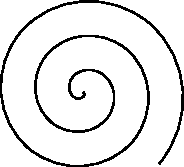
\includegraphics[width=8cm]{pics/spiral.pdf}
\caption{A spiral... smooth vector-based with a clean parametrisation! \\ Nothing to do with \cite{Gage:18}}\label{fig:spiral}
\end{figure}
\FloatBarrier

\section{Tables}

\begin{table}[H]
\small
\centering
\begin{tabular}{p{5cm}|l|p{3cm}}
`` Industrial era '' &  ``Jobs '' & `` Wanted: Upgrade''' \\ \hline
Parts exchanger & Fitter & mecatronics specialist \\
eShop & reseller & `` Client-suggester'' \\
`` Coding-guru''' & Softwaredesign & Whole-life designer \\
JA! Gut \& Günstig & brand-names & `` Life-Style Feeling'' \\
Internetbanking & Bank clerk & Customer adviser \\
Robots & Specialist & Machine supervisor \\
Bush & Gardener & Nature-sculptor \\
Painting & Painter & Interior Design \\
 &  & \\
\end{tabular}
\caption[Downgrade and upgrade of job denominations]{Downgrade and Upgrade of job denominations \\ \ \ \ \cite{DueckKo:2016}}
\label{tab:Downgrade and Upgrade of job denominations}
\end{table} 

\section{Listes}

\begin{itemize}
 \itemsep0pt
 \item one
 \item twoi
 \item threei
\end{itemize}

\begin{enumerate}
 \itemsep0pt
 \item first
 \item second
 \item third
\end{enumerate}


\section{Formulæ}

A formula can be written inline, e.g. as $ \frac{d}{dx}\mbox{arctg}(x) = \frac{1}{1+x^2}$ or, in centered math:

\begin{equation}  \frac{d}{dx}\mbox{arctg}(x) = \frac{1}{1+x^2} \label{arctanderivative}\end{equation}

Notice that formulæ that are centered start bigger (technically, they start in \verb+\displaystyle+) than they start inline (technically, they start in \verb+\textstyle+ all subsequents reductions, e.g. an exponent, goes to \verb+\scriptstyle+ then \verb+\scriptscriptstyle+). Indeed a best effort is made so that inline formulæ do not change the line height which would bother the eye of a reader.

Formulæ can be given a number and a label. Numbering happens automatically with \verb+\begin{equation}+ and \verb+\end{equation}+ and can be avoided if enclosing the formula betwee \verb+\[+ and \verb+\]+. If using the \verb+\label+ macro inside, you can refer automatically to this equation using \verb+\ref{label}+. E.g. Thanks to equation~\ref{arctanderivative} one dare say that:

\begin{equation} \int_0^t \frac{1}{1+x^2} dx = \mbox{arctan}(t) \end{equation}